In this chapter, theory related to multicore architecture and parallel programming is
explained in order to give the reader the foundation needed to understand these aspects of
the thesis. Also, the parallel capabilities of the Python programming language, including
drawbacks, are lined out. Finally, work related to this thesis is summarized in order to
utilize the conclusions drawn by others when solving problems similar to that of this thesis.

\section{Definitions}
\begin{itemize}
  \item \textbf{IPC} - Interprocess communication.
  \item \textbf{MPI} - Message Passing Interface. Standardized interface for message passing between processes.
  \item \textbf{Embarrassingly parallel} - A problem that is embarrassingly parallel can easily be broken down into components that
    can be run in parallel. %Cite astro? Python hpc?
  \item \textbf{CPU bound} - Calculation where the bottleneck is the time it takes for a processor to execute it.
  \item \textbf{I/O bound} - Calculation where the bottleneck is the time it takes for some input/output call, such as file accesses
    and network operations.
  \item \textbf{Real time} - The total time it takes for a call to finish.
  \item \textbf{User time} - The time a call takes, excluding system overhead; the time the call spends in user mode.
  \item \textbf{System time} - The time in a call that is consumed by system overhead; the time the call spends in kernel mode.
  \item \textbf{DAG/Directed acyclic graph} A directed graph that contains no directed cycles.
\end{itemize}

\section{Multicore architecture} %Find a better name?
\subsection{Processes vs threads}
while both threads and processes represent contexts in which a program is run, they have a few differences. A thread is run inside
a process, and the threads within the process share memory and state with each other and the parent
process \cite{singh_2013_parallel_padpwprfmm}. Individual processes do not share memory with each other, and any
communication between processes must be done with message passing rather than with shared memory. Consequently, communication
between threads is generally faster than between processes.
Typically, different threads can be scheduled on different cores, which is also true for different processes.

\subsection{Scheduling}
Threads and processes are scheduled by the operating system, and the exact mechanism for choosing what to schedule when differs
between platforms and implementations \cite[p. 472]{herlihy_2012_art_taomprr}. Scheduling may imply running truly parallel
on different cores, or on the same core using time-slicing. Threads and processes may be descheduled from running temporarily for several
reasons, including issuing a time-consuming memory request.

\subsection{Multicore communication and caching}
Multiple processors communicate with each other through a bus or a network \cite[p. 472-476]{herlihy_2012_art_taomprr}. Since the
means of communication between the processes is a finite resource, too much traffic may result in delays. The processors typically
have their own cache. In order to avoid unnecessary reads from the slower main memory, processors may read from another processor
that has the requested data cached. In a process called \emph{cache coherence}, shared cached values are kept up to date using one
of several protocols. The effect that these different means of communication between processors has on performance in
multiprocessor programs should not be ignored.

\subsection{Data parallelism}
Data parallelism denotes code where the parallelism comes from decomposing the data and running it with the same piece of code
across several processors or computers \cite{singh_2013_parallel_padpwprfmm}. It allows scalability as number of cores and problem
sizes increase, since more parallelism can be exploited for larger datasets \cite[p. 24]{mccool_2012_structured_spppfec}.

\subsection{Task parallelism}
In task parallelism, groups of tasks that are independent are run in parallel \cite{chow_2015_pipeline_ppiaote}.
Tasks that depend on each other cannot be run in parallel, and must instead be run sequentially.
A group of tasks is embarrassingly parallel if none of the tasks in the group depend on each other.

\section{Performance models for parallel speedup}

\subsection{Amdahl's law}
Amdahl's law \cite{amdahl_2013_computer_caaal} states that:
\begin{displayquote}
The effort expended on achieving high parallel processing rates is wasted unless it is
accompanied by achievements in sequential processing rates of very nearly the same magnitude.
\end{displayquote}

Amdahl divides programs into two distinct parts: a parallelizable part and an inherently
serial part
\cite[p. 13]{herlihy_2012_art_taomprr}.
If the time it takes for a single worker (for example, a process) to complete the program is $1$, Amdahl's law says
that the speedup $S$ of the program with $n$ workers with the parallel fraction of the program $p$ is:
\begin{displaymath}
  S = \frac{1}{1 - p + \frac{p}{n}}
  \label{amdahl}
\end{displaymath}

The law has the following implication: if the number of workers is infinite, the time it takes for a program to finish is still
limited by its inherently serial fraction. This is illustrated below:

\begin{displaymath}
  \lim_{n \to \infty} \frac{1}{1 - p + \frac{p}{n}} = \frac{1}{1 - p}
  \label{amdahl_lim}
\end{displaymath}

$1-p$ is the serial fraction which clearly limits the speedup of the program even with an unlimited number of processors.

\subsection{Extensions of Amdahl's law}
Che and Nguyen expand on Amdahl's law and adapts it to modern multicore processors \cite{che_2014_amdahl_alfmmp}. They find that
more factors than the number of workers affect the performance of the parallelizable part of a program, such as if the work is
more memory bound or CPU bound. In addition, they find that with core threading (such as hyperthreading), superlinear speedup of a
program is achievable and that the parallelizable part of a program is guaranteed to also yield a sequential term due to resource
contention.

Yavits et al. come to similar conclusions \cite{yavits_2014_effect_teocasoalims}. They find that it is important to minimize the
intensity of synchronization operations even in programs that are highly parallel.

\subsection{Gustafson's law}
Gustafson's law \cite{gustafson_1988_reevaluating_ral} is a result of the observation that problem sizes often grow with the
number of processors, an assumption that Amdahl's law dismisses, keeping the problem size fixed. With this premise, a program can
be run with a larger problem size in the same time as more workers are added. This view is less pessimistic than Amdahl's law, as
it implies that the impact of the serial fraction of a program becomes less significant with many workers and a large problem
size \cite[p. 61-62]{mccool_2012_structured_spppfec}.

The speedup $S$, for $n$ workers, and $s$ and $p$ as the time spent in the serial and parallel parts in the parallel system,
respectively, is achieved by:

\begin{displaymath}
  S = n + (1-n) * s
\end{displaymath}

\subsection{Work-span model} \label{work-span}
The tasks that need to be performed in a program can be arranged to form a directed acyclic graph, where a task that
has to be completed before another precedes it in the graph. The work-span model introduces the following terms
\cite[p. 62-65]{mccool_2012_structured_spppfec}:
\begin{itemize}
  \item \textbf{Work} - The work of a program is the time it takes to complete with a single worker, and equals the total time it
    takes to complete all of the tasks. The work is denoted $T_1$.
  \item \textbf{Span} - The span of a program is the time it takes for the program to complete with an infinite number of workers.
    The span is denoted $T_\infty$.
  \item \textbf{Critical path} - The tasks that are included in the path that has the maximum number of tasks that need
    to be executed in sequence. The span is equal to the length of the critical path.
\end{itemize}

An example of a task DAG can be found in figure \ref{fig:dag_example}.

\begin{figure}[ht]
  \centering
  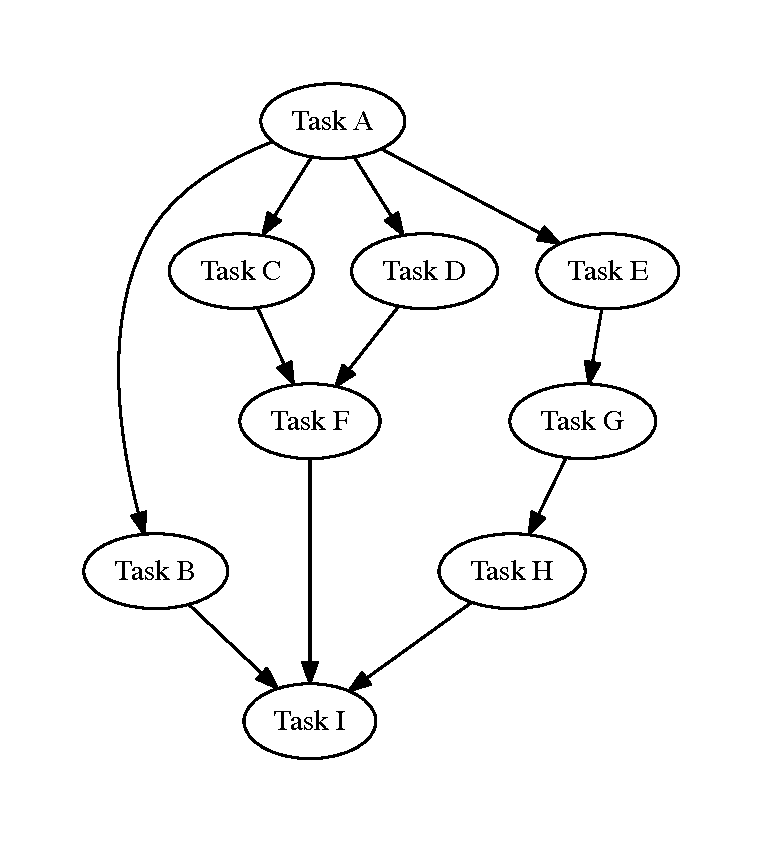
\includegraphics[width=120mm]{figures/task_dag_example.pdf}
  \caption[Example of work-span model task DAG]{An example of a task DAG used in the work-span model. Assuming each task takes
    time 1 to complete, this DAG has a \textit{work} of 9 and a \textit{span} of 5.}
  \label{fig:dag_example}
\end{figure}

In the work-span model, the following bound on the speedup $S$ holds:

\begin{displaymath}
  S \leq \frac{T_1}{T_\infty}
\end{displaymath}

With $n$ workers and running time $T_n$, the following speedup condition can be derived:
\begin{displaymath}
  S = \frac{T_1}{T_n} \approx P \text{ if } \frac{T_1}{T_\infty} \gg P
\end{displaymath}

In essence, this means that linear speedup can be achieved under the condition that the work divided by the span is significantly
larger than the number of workers.

The work-span model implies that increasing the work in an excessive manner when parallelizing may result in disappointing
results. It also implies that the span of the program should be kept as small as possible in order to utilize parallelization as
much as possible.

\section{Python performance and parallel capabilities}
There are several implementations of the Python language. This section will focus on CPython, the canonical and most popular
Python implementation, and also the one that TriOptima uses.

\subsection{Performance}
The general performance of CPython is slower than other popular languages such as C and Java for several
reasons \cite{barany_2014_python_pipd}. Overhead is introduced due to the fact that all operations need to dispatched dynamically,
and accessing data demands the dereferencing of a pointer to a heap data structure. Also, the fact that late binding is employed
for function calls, the automatic memory memory management in the form of reference counting, and the boxing and unboxing of
methods contribute to the at times poor performance.

\subsection{The GIL, Global Interpreter Lock}
In order to simplify the implementation and to avoid concurrency related bugs in the CPython interpreter,
a mechanism called the Global Interpreter Lock - or the GIL - is employed  \cite{palach_2014_parallel_ppwp}.
The GIL locks the entire CPython interpreter, making it impossible for multiple Python threads to make progress at
the same time, removing the benefits of parallel CPU bound calculations
\cite{glossary_gp2d}. When an I/O operation is started from Python, the GIL is released.
Efforts to remove the GIL have been made, but have as of yet been unsuccessful.

\subsection{Threading}
The Python \code{threading} module provides a multitude of utilities for concurrent programming, such as an object abstraction of
threads, locks, semaphores, and condition objects \cite{16_1thtip2d}. When using the \code{threading} module in CPython, the GIL is in
effect, not allowing true parallelism and hampering efficient use of multicore machines. When performing I/O bound operations, the
\code{threading} module can be used to improve performance; at times significantly \cite[p. 121-124]{slatkin_2015_effective_ep5swtwbp}

\subsection{Multiprocessing}
The \code{multiprocessing} module has a similar API to the \code{threading} module, but avoids the negative effects of the GIL by spawning
separate processes instead of user threads. This works since the processes have separate GILs, which do not affect each other and
enables the processes to utilize true parallelism \cite{slatkin_2015_effective_ep5swtwbp}. The processes are represented by the \code{multiprocessing.Process} class.

The \code{multiprocessing} module provides mechanisms for performing IPC.
In order for the data to be transferred between processes, it needs to be serializable through the use of the Python \code{pickle}
module \cite[p. 143]{slatkin_2015_effective_ep5swtwbp}. When transferring data, it is serialized, sent to another process through
a local socket, and then deserialized. These operations, in conjunction with the creation of the processes, gives the
\code{multiprocessing} module a high overhead when performing IPC.

The two main facilities that the \code{multiprocessing} module provides for IPC are \cite{palach_2014_parallel_ppwp}:
\begin{itemize}
  \item \code{multiprocessing.Pipe}, which serves as a way for two processes to communicate using the operations \code{send()}
    and \code{recv()} (receive). The Pipe is represented through two connection objects which correspond to each end of the pipe.
    See figure \ref{fig:code_pipe_example} for an example.
  \item \code{multiprocessing.Queue}, which closely mimics the behaviour and API of the standard Python \code{queue.Queue}, but
    can be used by several processes at the same time without concurrency issues. This \code{multiprocessing} queue internally
    synchronizes access by multiple processes using locks, and uses a \emph{feeder thread} to transfer data to other processes.
    See figure \ref{fig:code_queue_example} for an example.
\end{itemize}

In addition to the parallel programming utilities mentioned above, the \code{multiprocessing} module provides the \code{Pool} abstraction
for specifying a number of workers as well as several ways of assigning functions for the workers to be performed in parallel. For
example, a programmer can use \code{Pool.map} to make the workers in the pool execute a specified function on each element in a
collection.
See figure \ref{fig:code_pool_example} for an example.

\begin{figure}[ht]
  \centering
  \pythonexternal{code_examples/pipe_example.py}
  \caption{\code{multiprocessing.Pipe} example}
  \label{fig:code_pipe_example}
\end{figure}

\begin{figure}[ht]
  \centering
  \pythonexternal{code_examples/queue_example.py}
  \caption{\code{multiprocessing.Queue} example}
  \label{fig:code_queue_example}
\end{figure}

\begin{figure}[ht]
  \centering
  \pythonexternal{code_examples/pool_example.py}
  \caption{\code{multiprocessing.Pool} example}
  \label{fig:code_pool_example}
\end{figure}

\section{Related work} \label{related_work}
\subsection{Efficient parallelization of path planning workload on single-chip shared-memory multicores}
Ahmad et al. \cite{ahmad_2015_efficient_epoppwossm} parallelize path planning algorithms such as Dijkstra's algorithm using C/C++ and
Python in order to compare the results and evaluate each language's suitability for parallel computing. For the Python implementation,
both the \code{multiprocessing} and \code{threading} packages are used. The authors identify Python as the preferable choice 
in application development, due to its safe nature in comparison to C and C++. The implementation using the \code{threading}
module resulted in no speedup over the sequential implementation. Parallelization using the \code{multithreading} module resulted
in a speedup of 2.5x for sparse graphs, and a speedup of 6.5x for dense graphs. The overhead introduced by the interpreted nature
of Python, as well as the extra costs associated with Python multiprocessing, was evident as the C/C++ implementations showed both
better performance and better scalability. The slowdowns for sparse graph of Python compared to C/C++ ranged between
20x to 700x depending on the graphs.
However, the authors note that the parallel Python implementation exhibits scalability in comparison to its sequential implementation.

The experiments were conducted on a machine with 4 cores with 2-way hyperthreading.


\subsection{Harnessing multicores: Strategies and implementations in ATLAS}
Binet et al. \cite{binet_2010_harnessing_hmsaiia} present a case study where parts of the ATLAS software used in
LHC (Large Hadron Collider) experiments are parallelized. Because of the complexity and sensitivity of the system,
one of the goals of the study is to minimize the code changes when implementing the parallelization. The authors highlight several
benefits of using multiple processes with IPC (interprocess communication) instead of traditional multithreading, including ease of 
implementation, explicit data sharing, and easier error recovery. The Python \code{multiprocessing} module was used to parallelize
the program, and the authors emphasize the decreased burden thanks to not having to implement explicit IPC and synchronization.
Finding the parts of the program that is embarrassingly parallel and parallelizing these is
identified as the preferred approach in order to avoid an undesirably large increase in complexity while
still producing a significant performance boost.

The parallel implementation was tested by measuring the user and real time for different numbers of processes.
These measurements show a clear increase in user time because of additional overhead, but also a steady decrease in real time.

\subsection{On the Performance of the Python Programming Language for Serial and Parallel Scientific Computations}
Cai et al. \cite{cai_2005_performance_otpotpplfsapsc} note that Python is suitable for scientific programming thanks to its richness and
power, as well as its interfacing capabilities with legacy software written in other languages. Among other experiments on Python
efficiency in scientific computing, its parallel capabilities are investigated. The Python MPI package \code{Pypar} is used for
the parallelization, using typical MPI operations such as send and receive. The calculations, such as wave simulations, 
are made with the help of the \code{numpy} package for increased efficiency. The authors conclude that while communication 
introduces overhead, Python is sufficiently efficient for scientific parallel computing.

\subsection{Parallel astronomical data processing with Python: Recipes for multicore machines}
Singh et al. \cite{singh_2013_parallel_padpwprfmm} present Python as a fitting language for parallel computing, and use the
\code{multiprocessing} module as well as the standalone \code{Parallel Python} package in their experiments. Because of the
communication overhead in Python, the study focuses on embarrassingly parallel problems where little communication is needed.
Different means of parallelization are
compared: the Pool/Map approach, the Process/Queue approach, and the Parallel Python approach. 
In the Pool/Map approach, the simple functions of \code{multiprocessing.Pool} is used to specify a number of processes, a data
set, and the function to be executed with each element in the dataset as a parameter. In the Process/Queue approach, a
\code{multiprocessing.Queue} is spawned and filled with chunks of data. Several \code{multiprocessing.Process} objects are then
spawned, which all share the queue and get data to operate on from it while it is not empty. Another shared queue is used for
collection the results. In the Parallel Python approach, the \code{Parallel Python} abstraction \emph{job server}
is used to submit tasks for each data chunk. The tasks are automatically executed in parallel by the job server, and the results
are collected when they have finished.

The results in general show significant time savings even though the approaches taken are relatively straightforward.
The best performance is achieved when the number of processes is equal to the number of physical cores on the computer.
The Process/Queue is shown to perform better than both Pool/Map and parallel Python. This comes at the cost of a slightly less
straightforward implementation. The impact of load balancing and chunk size is also discussed, with the conclusion that work load
should be evenly distributed among cores as computation is limited by the core that takes the longest to finish.

\subsection{Parallel optimal choropleth map classification in PySAL}
Rey et al. \cite{rey_2013_parallel_pocmcip} compare \code{multiprocessing} and \code{Parallel Python} with the GPU-based parallel
module \code{PyOpenCI} when attempting to parallelize portions of the spatial analysis library PySAL. In particular, different
versions of the Fisher-Jenks algorithm for classification are compared. For the smallest sample sizes, the overhead of the
different parallel implementations produce slower code, but as the sample sizes grow larger the speedup grows relatively quickly.
For the largest of the sample sizes, the speedup curve generally flattens out; the authors state this as counter-intuitive and
express an interest in investigating this further. In general, the CPU-based modules \code{multiprocessing} and \code{Parallel Python}
perform better than the GPU-based PyOpenCI. The \code{multiprocessing} module produced similar or better results than the
\code{Parallel Python} module.
While the parallel versions of the algorithm perform better, the bigger implementation effort associated with it is noted.

\subsection{PEP 0371}
In their proposal for the inclusion of the \code{multiprocessing} module into the Python standard library,
Noller and Oudkerk \cite{noller_pep_p0} include several benchmarks where the \code{multiprocessing} module's performance is
compared to
that of the \code{threading} module. They emphasize the fact that the benchmarks are not as applicable on platforms with slow forking
time. The benchmarks show that while of course slower than sequential execution, \code{multiprocessing} performs better than
\code{threading} when just spawning workers and executing an empty function. For the CPU-bound task of computing Fibonacci numbers,
\code{multiprocessing} shows significantly better result than \code{threading} (which is in fact slower than sequential code). For I/O bound
calculations, which is an application considered suitable for the \code{threading} module, the \code{multiprocessing} module is still shown to have
the best performance when 4 or more workers are used.

The benchmarks where performed using the following hardware:
\begin{itemize}
  \item 4 Core Intel Xeon CPU @ 3.00GHz
  \item 16 GB of RAM
  \item Python 2.5.2 compiled on Gentoo Linux (kernel 2.6.18.6)
  \item pyProcessing 0.52
\end{itemize}

\subsection{Three Unique Implementations of Processes for PyCSP}
Friborg et al. \cite{friborg_2009_three_tuiopfp} explore the use of processes, threads and greenlets in their process abstraction
library PyCSP. The authors observe the clear performance benefits of using multiprocessing over threads due to the circumvention of the GIL
that the \code{multiprocessing} module allows. Greenlets are user-level threads that execute in the same thread and are unable to utilize
several cores. On Microsoft Windows, where the fork() system call is not available, the process creation is observed as
significantly slower than on UNIX-based platforms. While serialization and communication has a negative impact on performance when
using \code{multiprocessing}, the authors state that this produces the positive side-effect of processes not being able to
modify data received from other processes.

\subsection{Summary of related work}
Common themes and conclusions in the related work presented above include:

\begin{itemize}
  \item Python is a suitable language for parallel programming.
  \item The \code{multiprocessing} module is successful in circumventing the GIL and often shows the same or better performance than other
    methods, even for I/O bound programs.
  \item The overhead that IPC introduces when creating parallel Python programs makes it imperative to minimize communication and
    synchronization. Consequently, embarrassingly parallel programs are preferable when using Python.
  \item For existing larger systems, extensive parallelization may produce undesired complexity.
\end{itemize}
